%--------------------------------------------%
% Template Beamer para Apresentações da UFRN %
% by alcemygvseverino@gmail.com              %
% Baseado em MIT Beamer Template			 %
% versao 1.1								 %
% Atualizado em 14/05/2016					 %
%--------------------------------------------%
%\documentclass[handout,t]{beamer}
\documentclass[presentation,t]{beamer}
% Para alterar a linguagem do documento
\usepackage[portuges]{babel}
% Para aceitar caracteres especias deretamente do teclado
\usepackage[utf8]{inputenc}
% Para seguir as normas da ABNT de citacao e referencias
\usepackage[alf]{abntex2cite}
% Para incluir figuras
\usepackage{graphicx}
% Para melhor ajuste da posisao das figuras
\usepackage{float}
% Para ajustar as dimensoes do layout da pagina
\usepackage{geometry}
% Para formatar estrutura e informacoes de formulas matematicas
\usepackage{amsmath}
% Para incluir simbolos especiais em formulas matematicas
\usepackage{amssymb}
% Para incluir links nas referencias
\usepackage{url}
% Para incluir paginas de documentos .pdf externos
\usepackage{pgfpages}
% Para ajustar o estilo dos contadores
\usepackage{enumerate}
% Para modificar a cor do texto
\usepackage{color}
% Para incluir condicoes
\usepackage{ifthen}
% Para colocar legendas em algo que nao e float
\usepackage{capt-of}
% Pacotes para escrever algoritmos em pseudocódigo
\usepackage[portuguese, ruled, linesnumbered]{algorithm2e}
% Para definir o tema do slide
\usetheme{Berlin}
% Para difinir cores e background
\usecolortheme{ufrn}
% Para numerar as figuras
\setbeamertemplate{caption}[numbered]

% Título
\title[DIM0319]{Algoritmo e Programação de Computadores}
% Data
\date{\today}
% Autores
\author[Valdigleis]{Valdigleis\inst{1}}
	%\vspace{0.25cm}
	%Autor 02 \inst{2}
%}

% Instituto
\institute[UFRN]{
	\inst{1}%
        Universidade Federal do Rio Grande do Norte\\
        Centro de Ciência Exatas e da Terra\\
        Departamento de Informática e Matemática Aplicada\\
	\url{valdigleis@dimap.ufrn.br}\\
	\vspace{0.25cm}
	%\inst{2}%
	%Departamento\\
}

% Logo do canto inferior direito
\pgfdeclareimage[height=0.7cm]{logo_UFRN}{figuras/logo_UFRN}
\logo{\vspace*{-0.25cm}\pgfuseimage{logo_UFRN}\hspace*{-0.05cm}}


\begin{document}
% Sumário
\frame{\titlepage}
\section[]{}
\begin{frame}{Sumário}
	\tableofcontents
\end{frame}

% seções
\section{Apresentação da disciplina.}

\begin{frame}{Ementa da disciplina}
  \begin{enumerate}
    \item Descrição de Algoritmos.
    \item Construção de Algoritmos.
    \item Estudo dos recursos de alto nível com foco em Python: Variáveis, Tipos, Comandos, Subprogramas, Arquivos.
    \item Desenvolvimento sistemático de programas.
    \item Modelagem de problemas e suas respectivas resoluções através do uso de bibliotecas em Python.
  \end{enumerate}
\end{frame}

\begin{frame}{Metodologia usada e atendimento}
  \begin{itemize}
    \item Aulas expositivas utilizando quadro negro e projetor multimídia.
    \item Resolução (em sala de aula) de problemas. 
    \item Realização de atividades extraclasse na forma de listas de exercícios e/ou desafios de implementação.
  \end{itemize}
  \pause
  \begin{itemize}
    \item Horários de atendimento: \textbf{2T56} e \textbf{4M3456}.
  \end{itemize}
\end{frame}

\begin{frame}{Procedimentos de avaliação adotados}
  \begin{itemize}
    \item Primeira unidade: Prova escrita.
    \item Segunda unidade: Trabalho de implementação + lista de exercício.
    \item Terceira unidade: Trabalho de implementação + lista de exercício.
  \end{itemize}
\end{frame}
\section{Introdução informal para os algoritmos.}

\begin{frame}{Algoritmo?}
  Existem diversas definições dadas à palavra \textbf{algoritmo} (palavra derivada do nome Al-Khwarizmi), entre elas estão:
  \begin{itemize}
    \item Um procedimento passo a passo para a solução de um problema.
    \item Uma sequência detalhada de ações a serem executadas para resolver um problema.
    \item Raciocínio estruturado e finito para solucionar um problema.
  \end{itemize}
\end{frame}

\begin{frame}{Exemplo 01}
  \begin{itemize}
    \item Problema: Encontrar o livro de cálculo dentro do seu quarto.
  \end{itemize}
  \pause
  \begin{enumerate}
    \item Checar sua mochila.
    \item Verificar nos moveis (escrivaninha, guarda-roupa, e etc.).
    \item Olhar debaixo da cama.
    \item Se achou o livro, fique tranquilo.
    \item Se não achou o livro, aceite a derrota.
  \end{enumerate}
\end{frame}

\begin{frame}{Exemplo 02}
  Suponha que você tem acesso a dois recipientes, um com capacidade de 5 litros e outro com capacidade de 3 litros, além disso, você tem total acesso a uma fonte de água!
  \begin{itemize}
    \item Problema: Usando apenas os seus recipientes como é possível obter exatamente 7 litros de água?
    \pause
    \item {\color{red} Desafio}: No mesmo cenário anterior descreva como é possível obter exatamente 4 litros de água.
  \end{itemize}
\end{frame}


\section{Como representar algoritmos?}


\section{Relação: Algoritmos x Programas}

\begin{frame}{Sobre o computador}
  O que é um computador?
  \pause
  \begin{itemize}
    \item Uma máquina abstrata com uma fita (memória) infinita e um conjunto finito de regras de manipulação da fita \cite{turing1938computable}.
    \pause
    \item Um dispositivo eletrônico com uma memória finita, uma unidade central de processamento com um conjunto finito de instruções e dispositivos de entrada e saída para coleta e repasse de informação\cite{medina2006algoritmos}.
  \end{itemize}
  \pause
  \begin{figure}
    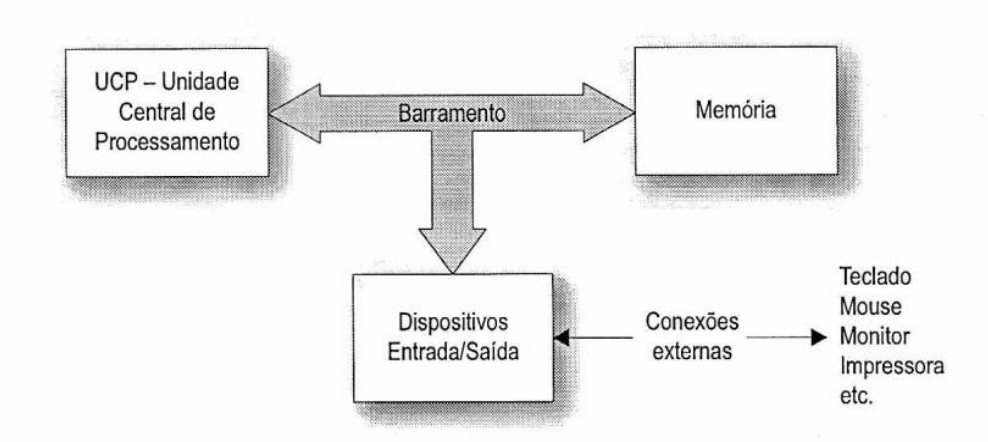
\includegraphics[width=0.5\textwidth]{figuras/Arquitetura.png}
  \end{figure}
\end{frame}


\begin{frame}{Sobre programas}
  O que é um programa?
  \begin{itemize}
    \item Uma sequência finita de instruções a serem executadas pela unidade central de processamento \cite{medina2006algoritmos}.
    \item É um algoritmo escrito em um formato compreensível pelo computador \cite{apostila2023}.
  \end{itemize}
\end{frame}



\begin{frame}{Referências}
  \bibliography{referencias}
\end{frame}

\end{document}
